\chapter{Motivation}
\url{https://github.com/NeverL8/ADL/tree/main/B06}\vspace{1cm}\newline
Previously we have used GANs in order to generate samples, i.e. numbers, based on the MNIST dataset. The adversarial approach of GANs with
a discriminator trying to identify fake images has some critical downsides. Convergence is not guaranteed, there is no inherent evalution metric
for sample quality and the generator can fall into mode collapse (only generating a few kinds of samples).
Diffusion models on the other hand do not require adversarial training, are parallelizable and scalable and promise converge in a stable manner.
They are based on gradual Markov chain noise generation in a forward process and are trained to predict the
added noise in a backward process (denoising).
Conclusively, the computational cost of diffusion models is extremly high, which is why we are only working on a rather simple problem here, i.e.
generating samples following a bimodal distribution of two gaussians.
\chapter{Code architecture}
The following hyperparameters are used:
\begin{minted}{python}
TIME_STEPS = 250
BETA = torch.tensor(0.02)
N_EPOCHS = 1000
BATCH_SIZE = 128
LEARNING_RATE = 0.8e-4
optimizer=torch.optim.Adam(g.parameters(), lr=LEARNING_RATE)
loss_function = torch.nn.MSELoss()
\end{minted}
Usually U-nets are used for diffusion models and in particular image generation. As just a single value is predicted in this exercise, a simple MLP is presumed to suffice. 
The following network with two hidden layers with 256 neurons each as well as ReLu activations is used:
\begin{minted}{python}
g = torch.nn.Sequential(
    torch.nn.Linear(2, 256), 
    torch.nn.ReLU(),
    torch.nn.Linear(256, 256),
    torch.nn.ReLU(),
    torch.nn.Linear(256, 1)
)
\end{minted}
Algorithm 1 and 2 are implemented for the forward and backward passes as given in \cite{paper}.
The implementation is given in the following. For explanation see the comments given in the code.
\begin{minted}{python}
    batches = range(0,shuffled_dataset.shape[0]-BATCH_SIZE, BATCH_SIZE)
    for i in batches:
        # sample a batch of data
        x0 = shuffled_dataset[i:i + BATCH_SIZE] #step 2

        # here, implement algorithm 1 of the DDPM paper 
        # (https://arxiv.org/abs/2006.11239)
        t = torch.randint(0,TIME_STEPS,(BATCH_SIZE,)) # sample timestep (step 3)
        epsilon = torch.randn_like(x0) # sample Gaussian noise
        # with same shape as x0 (step 4)
        alpha_bar_t = alpha_bars[t]

        x_t = (torch.sqrt(alpha_bar_t)*x0+torch.sqrt(1-alpha_bar_t)*epsilon) 
        # q(x_t | x_0) (forward)

        t_input = t.float()/TIME_STEPS # normalize
        input = torch.stack([x_t, t_input], dim=1) # stack sample values
        # and time steps together as network input

        predict_epsilon = g(input).squeeze() # squeeze: 
        #(batch size,1) -> (batch size) # step 5
        loss = loss_function(predict_epsilon, epsilon) # calculate loss # step 5

        optimizer.zero_grad() # ´clear old gradients
        loss.backward() # compute gradients
        optimizer.step() # update parameters

        train_loss += loss.item() # add loss to total loss for current epoch
        #-----------------
    train_loss=train_loss/len(batches)
    train_loss_hist.append(train_loss)
    
    # compute the loss on the validation set
    g.eval()
    with torch.no_grad(): # no operation tracking
        #for gradient computation -> only evaluation
        x0 = dataset_validation
        #--- same as for training
        t = torch.randint(0,TIME_STEPS,(x0.shape[0],))
        epsilon = torch.randn_like(x0) 
        alpha_bar_t = alpha_bars[t]
        xt = (torch.sqrt(alpha_bar_t) * x0 + torch.sqrt(1 - alpha_bar_t) * epsilon) 
        t_input = t.float() / TIME_STEPS
        input = torch.stack([xt, t_input], dim=1)
        predict_epsilon = g(input).squeeze()
        #----------
        val_loss = loss_function(predict_epsilon, epsilon)
    val_loss_hist.append(val_loss)
    epochs.set_description(f"Training loss = {train_loss:.2f},
    Validation loss = {val_loss:.4f}") # print losses next to progress bar
\end{minted}

\chapter{Results and observations}
The training converges quite quickly, with loss saturating after roughly 10 epochs (out of 1000) already as seen in \autoref{fig:loss}.
\begin{figure}
        \centering
        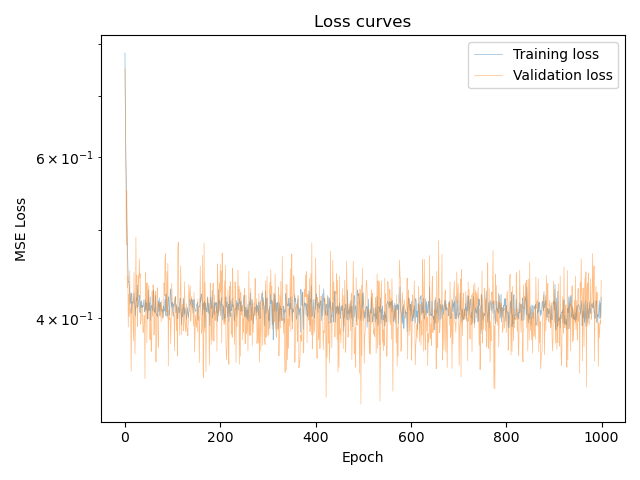
\includegraphics[width=\textwidth]{images/fullLossCurve.png}
        \caption{Epochs vs training and validation loss.}
        \label{fig:loss}
\end{figure}
A quick check reveals that the distributions of generated samples look similar after 20 epochs as they do after 1000, but since
this do not give us any further insight we will omit the results for 20 epochs here.
The distribution of generated samples at different timestep is displayed in \autoref{fig:time_evo}.
\begin{figure}
        \centering
        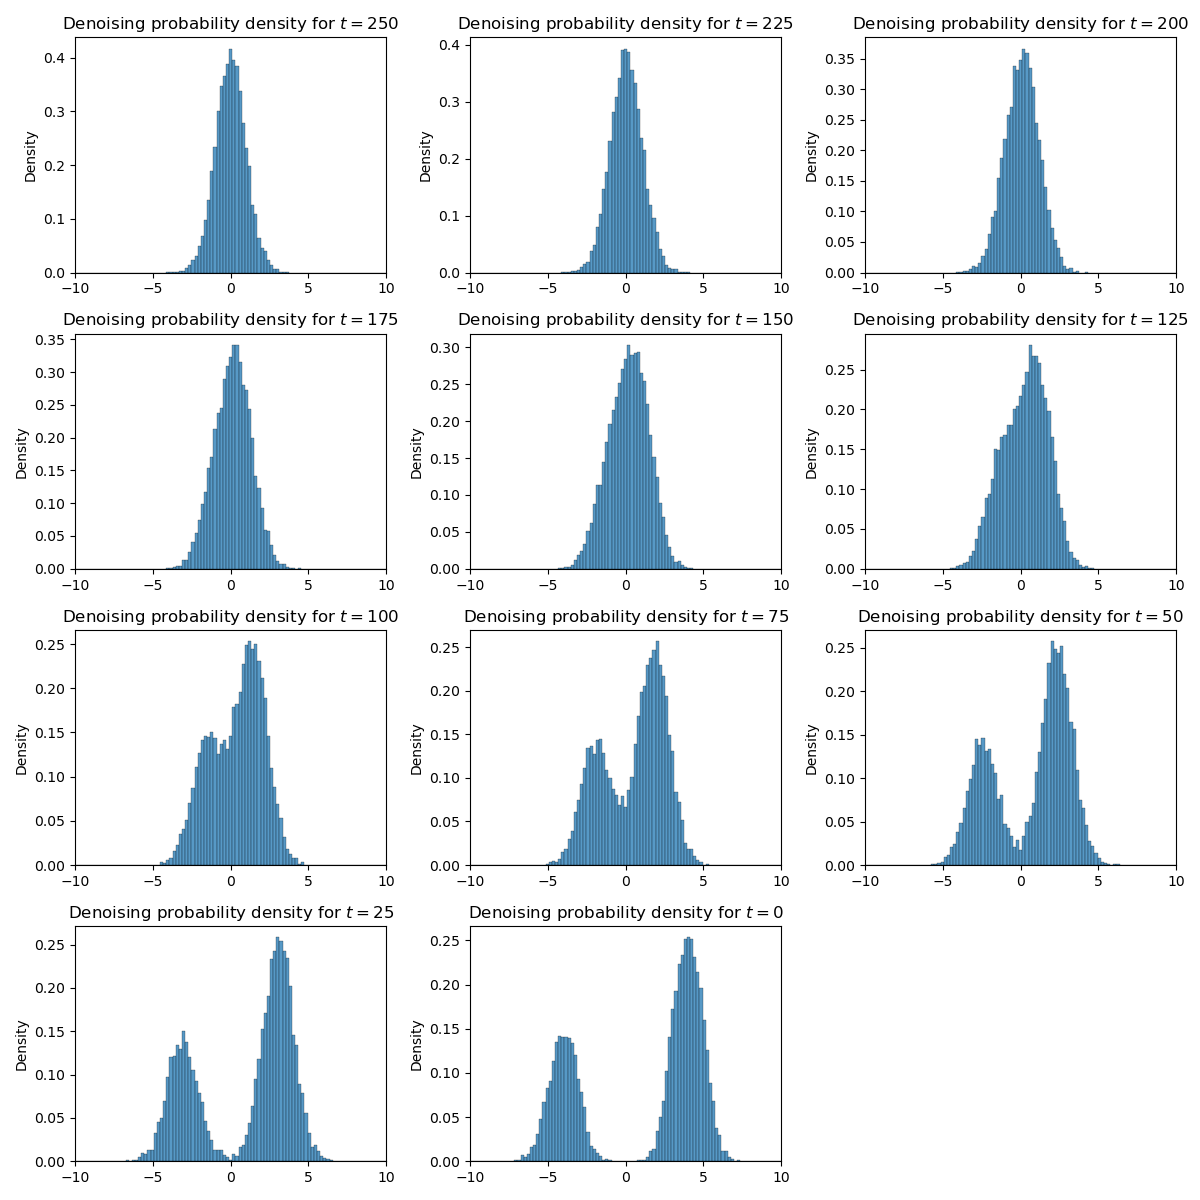
\includegraphics[width=\textwidth]{images/time_evolution.png}
        \caption{Sample distributions at different timesteps with $t=0$ being ideally completely denoised.}
        \label{fig:time_evo}
\end{figure}
One can observe that at roughly $t=100$ the bimodality of the distribution starts to emerge with clear separation of the individual gaussians only below $t=25$.
When plotting against the true distribution (see \autoref{fig:sampled_vs_true}) one finds that the positions of the peaks are almost reproduced perfectly.
However, the variance is reduced relative to the true distribution, which can be seen from the sampled distributions being higher than
the true distribution and lower than the true distribution in the tails. A large sample size of 50000 is chosen in order to ensure
that the deviations are not attributed to the binning.
\begin{figure}
        \centering
        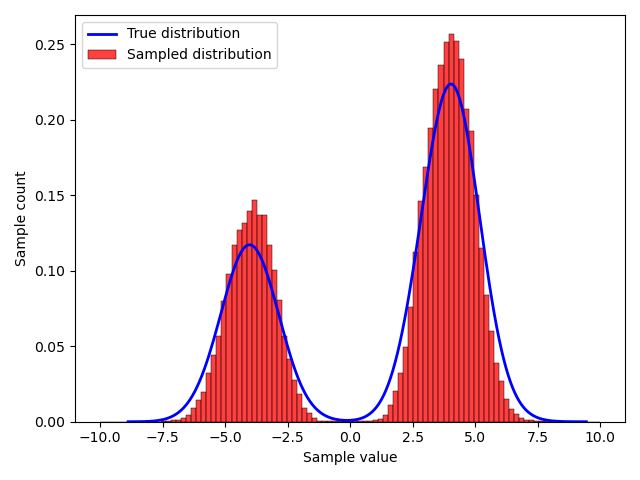
\includegraphics[width=\textwidth]{images/true_vs_sampled.png}
        \caption{Sampled distributions vs true distribution at $t=0$.}
        \label{fig:sampled_vs_true}
\end{figure}
The deviations can be quantified with means $\mu$ and standard deviations $\sigma$. For the calculation we look at the sampled values $x\leq0$ and $x>0$ separatetly, which is presumed to
suffice here, since the two gaussians appear to be well-separated.
The results are:
\begin{align*}
    \mu_{\leq0}= -3.96\\
    \sigma_{\leq0}= 0.95\\
    \mu_{>0}= 3.99\\
    \sigma_{>0}= 0.96,\\
\end{align*}
thereby veryfing our observations from the plot. As a reminder: The original distribution consists of two standard gaussians with means $-4$ and $4$ respectively.
\chapter{Conclusion}
One can conclude that the perk of diffusion networks being reliable and converging quickly has definitely proven to be
correct here with convergence after already $\~10$ epochs. The distribution is gradually "recovered" in the denoising process and
a distribution similar to the true dsitribution is found in the final timestep. Hence, the results are overall satisfactory and
match our expectations.
The only issue arising is the underestimation of the variance. This is likely due to low-probabilitiy regions occuring less
frequently and thereby contributing less to total loss than high-probability regions, so that accuracy is less well-optimized as for high-probability regions.
A more complex network architecure and a different loss function (giving higher weights to low-probability regions) might remedy this issue.
